\documentclass[../Relazione.tex]{subfiles}

\begin{document}
\section{Analisi delle pagine}
Questa sezione è la più importante e corposa; analizzeremo nel dettaglio l'usabilità della Homepage, di alcune pagine più rappresentative del sito e la comunicazione di informazioni da parte di esso, nel suo insieme, verso l'utente.
    \subsection{Assi di comunicazione}
    Nei confronti del sito l'utente necessita di avere risposta alle seguenti domande, comunemente riconosciute come gli assi principali della comunicazione, le famose 5 W +1:
    \begin{itemize}
        \item \textit{Who?} - Chi rappresenta questo sito?
        \item \textit{What?} - Cosa offre il sito? Mostramelo.
        \item \textit{Where?} - In quale punto del sito sono arrivato?
        \item \textit{When?} - Quali sono le ultime novità? Quand'è l'ultima volta che è stato manutenuto?
        \item \textit{Why?} - Perché mai dovrei fermarmi su questo sito? Quali benefici mi porterà tornarci?
        \item \textit{How?} - Capito ciò di mio interesse, come faccio ad arrivarci?
    \end{itemize}
Tradotte nel web, le 6 W sono tutte fondamentali nella Homepage, mentre per le altre pagine del sito gli assi si dividono secondo \textbf{obbligatori} (Who, What) ed \textbf{opzionali} (Where, When, Why, How).
L'asse \textbf{Where} seppur opzionale e altamente consigliato ovunque.\vspace*{0,5cm} \\
Richiamati quindi all'attenzione gli assi informativi, possiamo iniziare l'analisi in modo ordinato partendo dalla pagina più importante: la \emph{Homepage}.

\newpage

    \subsection{Homepage}

    Di seguito come si presenta la pagina della \emph{Homepage} del sito NordEst Paintball nella sua interezza.

        \begin{figure}[!h]
            \centering
            \includegraphics[width=\textwidth]{img/sito/Homepage.png}
            \caption{\textbf{Homepage} - Capture completa - (\url{http://www.lagunapaintball.it/})}
            \label{fig:homepage}
        \end{figure}

    \subsection{Considerazioni Iniziali}
    Essendo la Homepage la pagina principale di un sito e lo \textbf{scanning} l'azione implicita che un utente fa in prima battuta all'arrivo nella pagina iniziale (escludiamo per ora il \textbf{deeplinking}), vediamo se la struttura di questa pagina lo facilita o meno.
    Innanzitutto per ottenere il 100\% delle informazioni su questa pagina l'utente ha bisogno di effettuare 1 scroll verticale (qui visibile: figura \textbf{\ref{fig:scroll}} e \textbf{\ref{fig:scroll2}}) e considerando la prima parte visibilmente riempita da immagini, ciò non favorisce assolutamente lo scanning informativo!\\
    {\footnotesize(Maggiori approfondimenti sulle immagini nella sezione apposita: \textbf{\ref{sec:img}})}

\newpage

        \begin{figure}[!h]
            \centering
            \includegraphics[scale=0.25]{img/sito/Homepage_meta1.png}
            \caption{Homepage in browser - Safari 10.1 - Prima metà}
            \label{fig:scroll}
        \end{figure}

        \begin{figure}[!h]
            \centering
            \includegraphics[scale=0.25]{img/sito/Homepage_meta2.png}
            \caption{Homepage in browser - Safari 10.1 - Seconda metà}
            \label{fig:scroll2}
        \end{figure}

    D'altra parte le informazioni visibili a seguito dello scroll sono ben strutturate:
        \begin{itemize}
            \item Il testo informativo è diviso per piccoli blocchi divisi uno dall'altro per favorirne la lettura;
            \item è presente un breve titolo ben evidenziato (uso di \textbf{bold}) prima e dopo i blocchi che richiama l'attenzione;
            \item le informazioni sono chiare! Fan capire che questo sito offre l'esperienza del gioco del Paintball, niente più niente meno.
        \end{itemize}
    Infine, richiamando la struttura ed il contenuto del testo della Homepage, è importante far notare che quanto appena descritto EVITA certamente l'odioso \textbf{{\emph{''Blonde Effect''}}}, ovvero una percezione errata delle informazioni a causa dei limiti del visitatore. Durante lo scan l'utente può percepire erroneamente alcune zone.\vspace*{0,3cm}

    {\footnotesize(Per un breve momento di svago ed ulteriori informazioni esplicative --> perchè \href{https://www.youtube.com/watch?v=DctVteQDRIM}{Blonde Effect} ?)}


    \subsection{Assi fondamentali}

    Per la Homepage è \textbf{necessario} soddisfare tutte le 5W + 1. Analizziamoli qui di seguito.

        \subsubsection{Who}
        La pagina risponde a tale domanda grazie ad un immagine che copre in pratica tutta la parte dell'header.
        È quindi molta chiaro il nome di chi rappresenta il sito mentre non è assolutamente chiara l'entità riferita a quel nome, ovvero la società sportiva che si evince solamente nel footer della pagina con tutti i dettagli ad essa riferita.\\
        È presente inoltre il vero logo rappresentativo del sito ma, già avendolo fatto presente come fattore secondario all'immagine dell'header, significa che non risulta subito allo scan della home; è oltrettutto posizionato in una parte sconsigliata della pagina (in alto a destra), quindi non in alto a destra dove è la corretta posizione.\\
        Altro fattore negativo: l'URL del sito non corrisponde al titolo dell'header ed al logo, inoltre nelle immagini statiche appena sotto il menù di navigazione orizzontale, è indicato un (probabilmente vecchio) indirizzo differente dall'attuale!\\
        Un utente che entra per la prima volta alla homepage difficilmente potrebbe notare tutti questi dettagli ma in caso contrario rimarrebbe alquanto disorientato.\\
        Nonostante le informazioni quindi ci siano, esse sono mal disposte ed il risultato è quindi insoddisfacente. L’utente deve risalire a tali informazioni solo aggiungendo sforzo per uno scroll al fondo.\\
        Mancante una sezione (che avrebbe potuto chiamarsi 'About us'' o 'Chi siamo'') per chiarire nel dettaglio, a richiesta dell'utente, chi gestisce il posto e l'organizzazione sportiva. (quella chiamata ''Contatti'' non è esaustiva)

        \subsubsection{What}
        Nella pagina risulta molto chiara l'offerta di questo sito: varie modalità ed esperienze di gioco del paintball all'interno della struttura appositamente creata.
        Son presenti 3 immagini statiche che mostrano situazioni reali di gioco per dimostrare all'utente la situazione effettiva in cui si troverebbe.\\
        Per quest'asse comunicativo quindi, la homepage comunica bene tutti i contenuti offerti dal sito adibendo alla sua principale funzione.

        \subsubsection{When}
        L'informazione riguardante quest'asse è completamente assente! Fattore decisamente grave.
        Non vi è alcuna informazione temporale riguardante le ultime novità, gli ultimi eventi svoltisi ne l'ultima manutenzione o aggiornamento dei contenuti del sito.\\
        L'unica cosa che potrebbe risultare un'informazione utile per gli utilizzatori sono i 3 link nell'header sotto al logo bianco, che rimandano a dei social dell'organizzazione (Facebook, Twitter, Youtube) come vediamo dall'immagine appena sotto.\\
        Sono 3 immagini riferite a link esterni e richiedono perciò maggiore sforzo ed inventiva all'utente, che potrebbe addirittura ignorarle!\\
        L'utente, per quest'asse informativa, non ha quindi nessun riferimento se non ipotizzare di trovare qualcosa tramite LINK ESTERNI per delle informazioni che dovrebbero essere fornite automaticamente senza ulteriori operazioni. (figuriamo uscendo dal sito stesso!).
        Molto male.

        \begin{figure}[!h]
            \centering
            
\includegraphics[scale=0.3]{img/sito/Where.png}
            \caption{Header dell'Homepage - Immagini linkate a social esterni al sito che potrebbero dare informazioni sulle ultime novità ed eventi del posto}
            \label{fig:label}
        \end{figure}

        \subsubsection{Why}
        Grazie alla presenza nel logo e nell'immagine che compone l'header, della parola \emph{Paintball}, l’utente capisce immediatamente l’ambito e le tematiche trattate dal sito.
        \textit{Perchè scegliere NordEst Paintball e non altre società}, è molto convincente in questa pagina, che svolge quindi bene questa funzione.\\
        Grazie alla descrizione a blocchi degli scenari e degli slogan in grassetto con font maggiore per risaltare l'attenzione al contesto reale e dedicato, l'utente è invogliato a leggere, informarsi ulteriormente ed eventualmente chiamare per una prenotazione.\\
        Unica nota da evidenziare è che la sezione \textbf{Eventi}, che rispecchia perfettamente quest'asse comunicativo, è distaccata dalla homepage quando si poteva dare introduzione, riferimenti ad essa o addirittura inglobarla a questa pagina sostituendo le immagini sotto il menù che sono la causa dello scroll aggiuntivo. È pur sempre una scelta personale dello sviluppatore/committente in base alle preferenze di contenuti ed ordine del sito.

        \subsubsection{Where}
        Abbastanza inconsistente anche questa parte informativa.
        L'utente, come unico riferimento spaziale all'interno della homepage, ha un'evidenziazione della scritta ''Home'' nella scheda associata del menù di navigazione orizzontale.
        Questo menù, essendo statico, non differisce nelle altre pagine del sito.\\
        Nonostante la logica semplice mi sento di dire che, per la tipologia e la struttura gerarchica semplice di questo sito, il \emph{breadcrump} presente, (più vicino alla tipologia \textbf{Attribute}, che mostra la categoria e gli attributi della pagina) è molto adatto.

        \subsubsection{How}
        Come già precisato, il menu di navigazione semplice composto di sole 6 voci garantisce all’utente l’accesso alle informazioni desiderate in modo chiaro ed immediato.\\
        Manca completamente una funzione di ricerca all'interno di questa pagina (e delle altre) che permetta di mirare le informazioni che l'utente ricerca a meno di una entrata al sito tramite \emph{deeplinking}.
        Forse, per la natura limitata di informazioni e pagine, essa non è stata prevista ma è sempre buona norma adottarla.

\newpage

    \subsection{Pagina interna - Eventi}

    Analizzeremo ora due pagine secondarie di maggiore importanza per lo scopo del sito; in ordine quella degli \textbf{Eventi} e quella del \textbf{Listino}.\\

    Da qui in poi alcuni assi risultano essere obbligatori per tutte le pagine interne, mentre altri diventano opzionali.

        \begin{figure}[!h]
            \centering
            \includegraphics[width=\textwidth]{img/sito/Eventi.png}
            \caption{Pagina \textbf{Eventi} - Capture completa - (\url{http://www.lagunapaintball.it/index.php/menu-eventi})}
        \end{figure}

    \subsubsection{Assi obbligatori}
        \vspace*{0,5cm}
        \begin{itemize}
            \item \textbf{\underline{Who}}
            \vspace*{5mm}\\Come per la homepage e come per tutte le altre pagine, l'immagine che compone l'intero header ed il logo rappresentano il sito.
            \item \textbf{\underline{What}}
            \vspace*{5mm}\\Cosa offre il sito è esattamente il contenuto informativo reso disponibile da questa pagina.\\ Le informazioni son raggruppate a blocchi, in modo ordinato disposte 2 a 2 formando un quadrato e facilitando l'assimilazione e lo scan utente.\\
            È prensente un titolo rosso con font molto grande che richiama il blocco e delle keyword in rosso per attirare subito all'informazione cercata.\\
            Nonostante quindi una buona struttura informativa, le info sono leggermente ambigue:
            \begin{itemize}
                \item La descrizione posizionata in \textbf{alto a sinistra} e quella \textbf{in basso a destra} sono chiaramente due tipologie di eventi per i game;
                \item Il contenuto in \textbf{alto a destra} non è la descrizione di un vero e proprio evento;
                \item Infine, in \textbf{basso a sinistra} è presente una minimappa indicante tutti i tipi di campi/scenari con una indicazione dimensionale della struttura, insomma una informazione del tutto diversa ad un evento.
            \end{itemize}

            In aggiunta a quanto detto, queste informazioni che un utente può facilmente assimilare durante lo scan o una lettura più approfondita, sono frutto di pure immagini contenenti tutte le scritte necessarie!!\\
            Ci troviamo di fronte ad un chiarissimo esempio di \textbf{metafora visiva}: queste immagini non sono inizialmente e sicuramente riconosciute come immagini, bensì come testo.
            Non è assolutamente presente in realtà del testo nel body di questa pagina e ciò è un aspetto gravissimo per la logica di costruzione del sito, oltre che per la sua usabilità!\\
            Proviamo a pensare se durante l'accesso ci fosse un interruzione del caricamento dei dati del sito dovuta ad eventuali problemi di rete: il testo è ovviamente il primo elemento che viene caricato alla richesta di un sito, mentre le immagini son di contorno o comunque se avvengono parallelamente (practice sbagliata) sono elementi più corposi da visualizzare.
            \textbf{La pagina si presenterebbe priva di qualsiasi contenuto informativo} come è mostrato dall'immagine (orrenda) seguente che simula questa interruzione:

            \begin{figure}[!h]
                \centering
                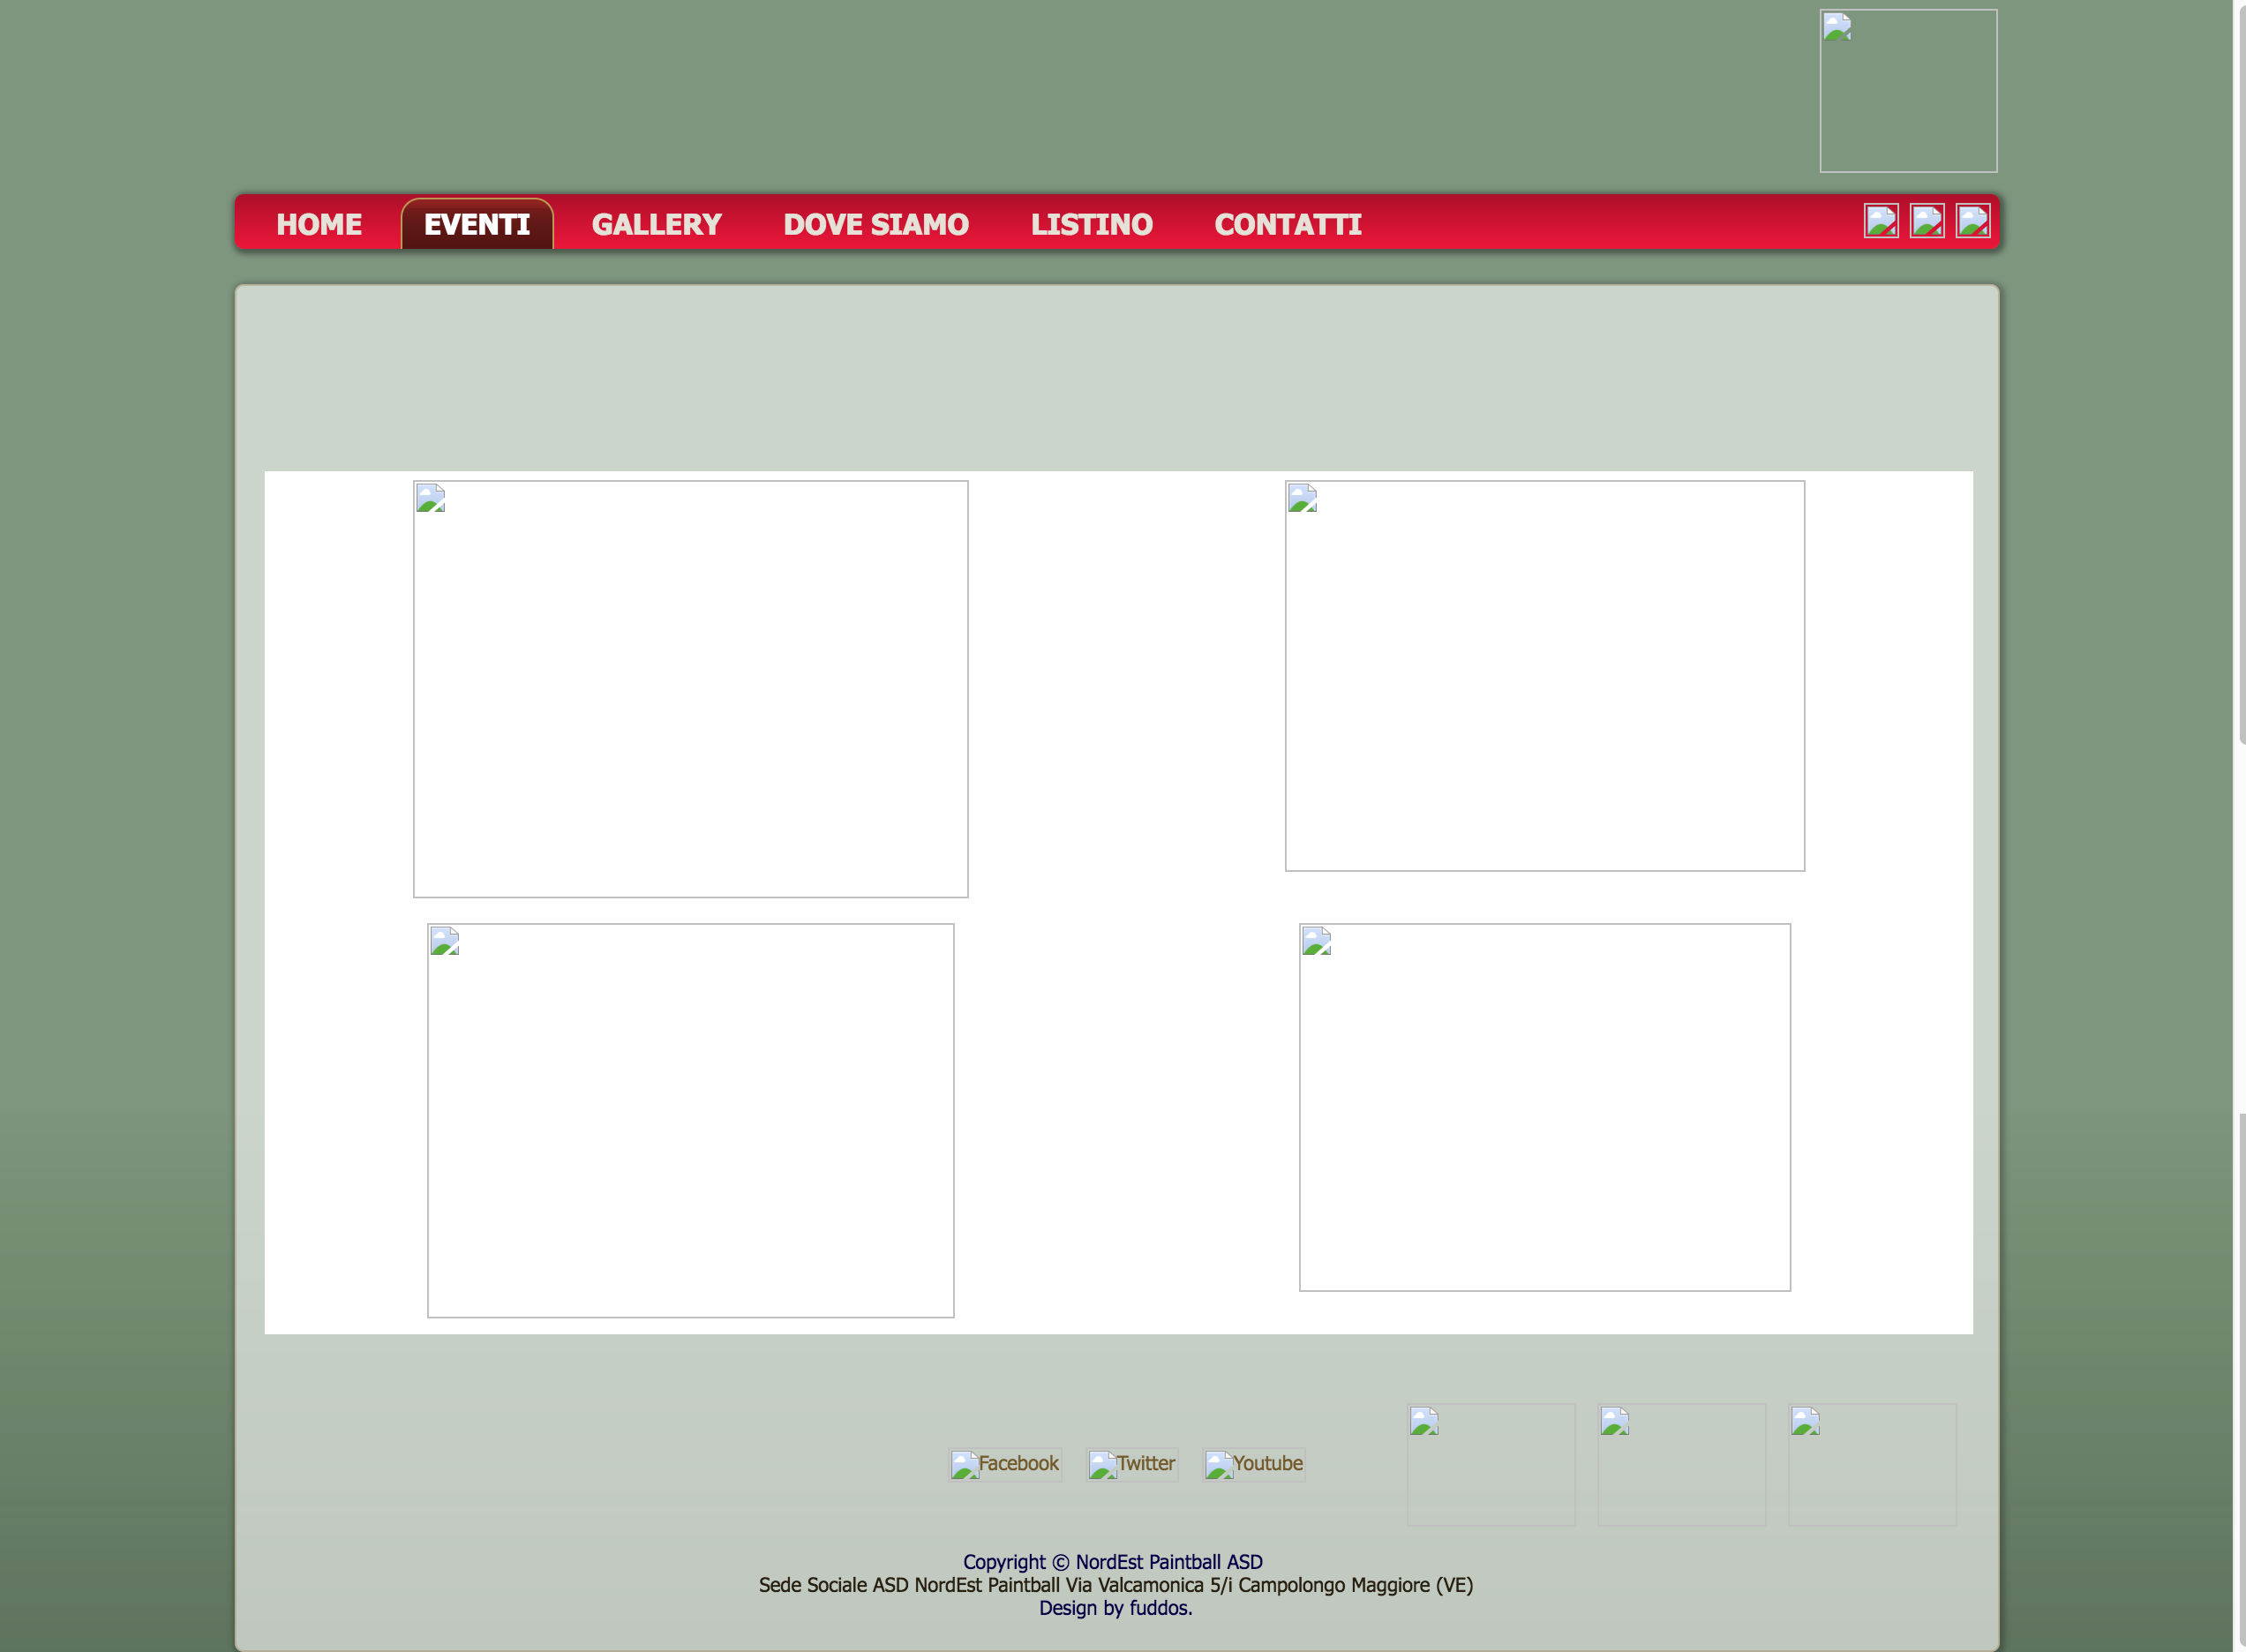
\includegraphics[width=0.6\textwidth]{img/sito/Eventi_noimage.png}
                \caption{Eventi - il caricamento interrotto prima che le immagini si carichino mostra come non esista alcuna informazione, molto grave!}
                \label{fig:noInfo}
            \end{figure}

        \end{itemize}

    \subsection{Assi opzionali}
        \vspace*{0,5cm}
        \begin{itemize}
            \item \textbf{\underline{Where}}
            \vspace*{5mm}\\Pur essendo un asse opzionale è consigliatissima poichè se assente l'utente sarà obbligato a tornare in home per maggiori informazioni orientative.
            In questa pagina come già evidenziato per la home ma anche come per tutte le altre pagine del sito, l'unico riferimento spaziale è un \emph{breadcrump} di tipo attribute che evidenzia nel menù orizzontale dell'header dove l'utente si trova.
            \item \textbf{\underline{When}}
            \vspace*{5mm}\\Come per la homepage e per tutte le altre pagine, anche in questa sezione continua ad essere assente un'informazione diretta sulle ultime news, esperienze o accessi di manutenzione!
            \item \textbf{\underline{Why}}
            \vspace*{5mm}\\La pagina stessa ha la funzione di fornire il perchè un utente dovrebbe scegliere di venire a giocare qua e le informazioni (anche se fornite tramite immagini) sono presenti, ben strutturate e chiare. Come sempre quest'asse informativo è soddisfatto contando soprattutto la natura del sito, che deve invogliare l'utente a prenotare i campi per provare/tornare a giocare.
            \item \textbf{\underline{How}}
            \vspace*{5mm}\\In questa pagina si fa sentire la mancanza di un riferimento (tramite link diretto o meno) ad una fonte di prenotazione, fondamentale per lo scopo di questo sito web!\\
            Sebbene sia presente una pagina \textbf{Contatti} che possiede il form per le richieste info e prenotazioni, ciò non basta in quanto l'utente non conosce a memoria il sito. Egli deve essere guidato con il minor numero di click ed il minor sforzo computazionale possibile per il raggiungimento del suo scopo, delle informazioni che intende avere e del come procurarsele nel minor spreco di risorse possibile.\\
            Continua anche in questa pagina ad essere assente una barra di ricerca.\\
            Asse non soddisfatto.

        \end{itemize}

\newpage
    \subsection{Pagina interna - Listino}

    Di seguito l'analisi della pagina dei listini per i vari tipi di ''pacchetti'' acquistabili.
        \begin{figure}[!h]
            \centering
            \includegraphics[width=\textwidth]{img/sito/Listino.png}
            \caption{Pagina \textbf{Listino} - Capture completa - (\url{http://www.lagunapaintball.it/index.php/menu-listino})}
        \end{figure}

    \subsubsection{Assi obbligatori}
        \vspace*{0,5cm}
        \begin{itemize}
            \item \textbf{\underline{Who}}
            \vspace*{5mm}\\Come detto già sopra, l'immagine che compone l'intero header ed il logo rappresentano il sito.
            \item \textbf{\underline{What}}
            \vspace*{5mm}\\Questa pagina segue la struttura informativa della pagina \emph{Eventi} descritta in precedenza. Le informazioni contenute descrivono molto dettagliatamente quanto ordinatamente le 4 tipologie di pacchetti che ogni singolo giocatore può scegliere (ovviamente uno al massimo) con associate le varie opzioni disponibili.\\
            Questa volta i blocchi informativi sono tutti coerenti, ovvero sono 4 sezioni di tipologia differente di pack, ma il problema della logica progettuale e la metafora visiva presente per la pagina degli \emph{Eventi} permane gravemente: tutte le informazioni scritte sono in realtà immagini statiche!
            Quindi, come per l'esempio prima, non sarà presente alcun contenuto scritto nel caso avvenisse un interruzione di rete prima del loading delle immagini.\\
            È presente un altro errore: senza un ulteriore scroll (quindi altro sforzo per l'utente) non si riesce a vedere un messaggio presente (sempre tramite una maledetta immagine) dopo la presentazione dei pacchetti; il messaggio specifica \emph{''Tessera AICS obbligatoria''}. È quindi un'informazione molto importante ai fini economici, in quando ha un costo escluso dal pacchetto (che un utente non informato non sa) ed un valore legale in quanto obbligo/regolamento della struttura.
            Grave mancanza anche questa nel non segnalarlo più chiaramente!
        \end{itemize}

    \subsection{Assi opzionali}
        \vspace*{0,5cm}
        \begin{itemize}
            \item \textbf{\underline{Where}}
            \vspace*{5mm}\\Anche in questa pagina, come già detto precedentemente per le altre, l'unico riferimento spaziale è un \emph{breadcrump} di tipo attribute che evidenzia nel menù orizzontale dell'header dove si trovo l'utente.
            \item \textbf{\underline{When}}
            \vspace*{5mm}\\Anche in questa pagina continua ad essere assente un'informazione diretta sulle ultime news, esperienze o accessi di manutenzione!
            \item \textbf{\underline{Why}}
            \vspace*{5mm}\\Esponendo svariate tipologie di pacchetti con prezzi differenti e adattati a diverse tipologie di giocatore (per allenarsi, per tutti e per i duri) fa si che l'utente possa scegliere in base alle sue esigenze, siano esse economiche, tecniche o fisiche.\\
            Purtroppo non è segnalato come munizioni aggiuntive e marcatori modificati (più grandi e precisi) siano selezionabili a parte ad un costo aggiuntivo.\\
            Queste informazioni di cui io sono al corrente per il fatto di aver giocato li, non sono percepibili da un nuovo utente, che solo al momento dell'esperienza concreta o tramite informazioni ottenute in modo traverso al sito, avrà.\\
            Ciò potrebbe causare in base di certo anche alla tipologia di utenza, qualche dispiacere o disagio che potrebbe portare a sconsigliare ad altri utenti questo sito, a dare recensioni non del tutto positive o peggio a non tornare più nel sito e all'esperienza di gioco; tutto poichè questi piccoli dettagli non sono inclusi inizialmente ad informazione completa per i clienti come dovrebbero.\\
            \item \textbf{\underline{How}}
            \vspace*{5mm}\\Anche in questa pagina è assente un riferimento di qualsiasi tipo ad una fonte di prenotazione o ad una procedura da seguire al fine di prenotare/acquistare. Molto male.\\
            Continua anche in questa pagina ad essere assente una barra di ricerca.\\
            Asse non soddisfatto.

        \end{itemize}
   

\end{document}
